\documentclass[twocolumn, 10pt]{article}
\usepackage[utf8]{inputenc}
\usepackage{graphicx}
\usepackage{amsmath}
\usepackage{hyperref}
\usepackage{geometry}
\geometry{margin=0.75in}

\title{SoundCLR Reproduction for Environmental Sound Classification}
\author{Project Team}
\date{\today}

\begin{document}

\maketitle

\begin{abstract}
Environmental Sound Classification (ESC) is a challenging task due to the high variability of audio signals and the limited size of labeled datasets \cite{piczak2015esc}. In this project, we reproduce key components of the SoundCLR framework, focusing on its most effective configuration \cite[Sec. IV]{soundclr}. Specifically, we implement a training pipeline combining transfer learning, strong data augmentation applied to both raw audio signals and spectrograms, and a three-channel input representation \cite[Sec. III-A]{soundclr}, alongside a hybrid deep network optimizing both cross-entropy and supervised contrastive losses. Our results closely match those reported in the original paper, with accuracy differences within $\pm 1\%$ across folds \cite[Fig. 4]{soundclr}. These small differences are expected due to stochastic training and the fact that the original results are averaged over multiple runs. Overall, our findings confirm both the effectiveness of the proposed training pipeline and the reproducibility of the SoundCLR approach under realistic computational constraints.
\end{abstract}

\section{Introduction}
Environmental Sound Classification (ESC) aims to automatically recognize sound events such as dog barks, rain, or engine noise. This task has many real-world applications, including surveillance systems, smart environments, and autonomous systems \cite{li2007robot, radhakrishnan2005audio, intani2013crime}. One of the main challenges in ESC is the relatively small size of labeled datasets, which makes training deep neural networks difficult and prone to overfitting. Recent research has shown that transfer learning and data augmentation can significantly improve performance in such settings \cite{salamon2017deep}.

The SoundCLR framework addresses these challenges by combining transfer learning from ImageNet-trained models, strong data augmentation applied to both raw audio and spectrogram representations, and a hybrid learning objective that combines cross-entropy and supervised contrastive loss \cite[Sec. III]{soundclr}. In this project, we aim to reproduce the key experimental findings of the paper. Due to computational limitations and the large number of experiments in the original work, we focus on the configurations that demonstrate the main contributions of the method \cite[Sec. IV]{soundclr}.

\section{Related Work}
Early ESC approaches relied on classical machine learning methods using handcrafted features. These approaches were later outperformed by deep learning models, particularly convolutional neural networks operating on spectrogram representations \cite{zhu2018learning}. 

Because training deep neural networks with millions of parameters requires large amounts of data, the comparatively small size of current ESC benchmark datasets makes applying data augmentation a necessity for learning effective networks \cite{tokozume2018learning, zhang2018deep}. 

Transfer learning has become a key technique in ESC, allowing models pretrained on large image datasets to be adapted for audio classification tasks. This is effective because spectrograms exhibit structural similarities to images. Another important direction is contrastive learning, which improves representation quality by explicitly encouraging separation between different classes in the embedding space \cite{khosla2020supervised}. SoundCLR combines these ideas into a unified framework, integrating transfer learning, strong augmentation, and a hybrid loss function \cite[Sec. III]{soundclr}.

\section{Method}
Our methodology reproduces the key components of the SoundCLR framework using a two-fold experimental structure. First, we independently implement and evaluate the proposed training pipeline \cite[Sec. III-A]{soundclr}---which incorporates transfer learning alongside strong data augmentation on both raw audio waveforms and spectrograms---to isolate its standalone influence on the model's accuracy. Second, utilizing the augmented representations generated by this pipeline, we aim to measure the impact of different loss functions on the final classification results \cite[Sec. III-C]{soundclr}. To this end, we train and compare the framework under three distinct learning strategies: (1) a baseline model trained strictly using cross-entropy for pure classification, (2) a two-stage decoupled network applying supervised contrastive learning followed by linear classification, and (3) a joint hybrid architecture optimizing both contrastive and cross-entropy losses simultaneously. Ultimately, this structured comparison allows us to verify the separated contributions of the data processing pipeline, while successfully confirming the reported superiority of the hybrid loss objective over the isolated classification and decoupled contrastive approaches.
\subsection{Architecture}
The core architecture is built upon a ResNet-50 backbone \cite{he2016deep} pretrained on ImageNet, acting as a shared feature extractor. The model receives 3-channel log-mel spectrograms (generated by triplicating a single audio channel) to fully utilize the pretrained visual weights. The output from the backbone's final layer produces a normalized high-dimensional representation vector. Beyond this feature extractor, the network structure explicitly diverges based on the three learning objectives:
\begin{itemize}
    \item \textbf{Cross-Entropy Classification:} The ResNet-50 backbone is followed by a single linear fully-connected classification layer. The output dimension of this layer corresponds discretely to the number of target classes. The model maps logits to predicted probabilities and computes standard categorical cross-entropy loss, formulated for a sample $i$ as:
    \begin{equation}
        \mathcal{L}_{\text{CE}_i} = -\sum y_{i} \log(\hat{y}_{i})
    \end{equation}
    where $y_{i}$ represents the one-hot encoded ground truth label and $\hat{y}_{i}$ is the predicted probability for the classes.

    \item \textbf{Supervised Contrastive Learning (Two-Stage):} In the representation stage, the classifier is replaced by a projection network consisting of a linear fully connected layer. This layer downsamples the representation vector into a lower-dimensional projection space optimized by supervised contrastive loss. For a mini-batch containing $N$ samples, where $N_{y_i}$ is the number of samples with identical labels to sample $i$, the loss is computed over the normalized projection vectors $z$ as:
    \begin{equation}
        \mathcal{L}_{\text{sup-con}_i} = -\frac{1}{N_{y_i}} \log \frac{\sum_{j=1}^{N} \mathbf{1}_{[y_i=y_j]} \exp(z_i \cdot z_j / \tau)}{\sum_{k=1}^{N} \mathbf{1}_{[k \neq i]} \exp(z_i \cdot z_k / \tau)}
    \end{equation}
    where $\tau$ is a temperature scaling hyperparameter. In the second evaluation stage, the backbone is frozen, and a linear classification layer is trained on top of the established representations using $\mathcal{L}_{\text{CE}}$.

    \item \textbf{Hybrid Loss Strategy:} The hybrid architecture routes the shared representation vectors through two parallel branches simultaneously: a linear classifier head computing cross-entropy, and a linear projection head computing supervised contrastive loss. This joint structure computes a combined loss weighted by hyperparameter $\alpha$ \cite[Sec. III-C]{soundclr}:
    \begin{equation}
        \mathcal{L}_{\text{hybrid}_i} = \alpha \mathcal{L}_{\text{sup-con}_i} + (1 - \alpha) \mathcal{L}_{\text{CE}_i}
    \end{equation}
    This allows synchronous end-to-end training over both objectives identically to the original SoundCLR configuration.
\end{itemize}

\subsection{Evaluation Metrics}
We evaluate performance using classification accuracy:
\begin{equation}
\text{Accuracy} = \frac{\text{Number of correct predictions}}{\text{Total number of samples}}
\end{equation}
Results are reported across folds to ensure robustness and consistency.

\subsection{Experimental Setup}
Our experiments are divided into two primary evaluations. To isolate and analyze the effect of the training pipeline components (transfer learning and data augmentation), we evaluate the model exclusively using the ESC-50 dataset with standard 5-fold cross-validation. Subsequently, to rigorously compare the effect of the various loss functions, as in the original paper, we expand our evaluation across three standard environmental sound datasets: ESC-50 evaluated over 5 folds, ESC-10 evaluated over 5 folds, and UrbanSound8K (US8K) \cite{salamon2014dataset} evaluated over 10 folds. Throughout all experiments, due to computational constraints, we focus on reproducing the specific network configurations that structurally demonstrate the main contributions and optimal states of the SoundCLR framework. We adopted the exact hyperparameters that yielded the best performance in the original paper, as our intention is to validate only the best results. Specifically, we use the Adam optimizer with 10 warm-up epochs and an exponential learning rate decay factor of $\gamma=0.98$. The base learning rate is set to $5 \times 10^{-4}$ for ESC-50 and ESC-10, and $1 \times 10^{-4}$ for US8K. The hybrid loss is governed by a temperature parameter $\tau=0.05$ and a weight calibration of $\alpha=0.5$. Spectrogram augmentations apply $f=2$ frequency masks and $t=1$ time mask, both with a maximum width of 32.

\subsection{Effect of Training Pipeline Components}
The original work demonstrates how components contribute to overall performance \cite[Fig. 3]{soundclr}. The configuration gradually adds transfer learning, multi-channel representation, and dual-domain data augmentation. Key conclusions indicate that transfer learning provides the largest improvement, showing that pretrained visual features transfer well to spectrograms. Using three input channels improves performance by enabling better use of pretrained weights. The best results are achieved only when all components are combined into a unified pipeline. Figure 1 presents our results of classification over the 5 folds of ESC-50 using the whole pipeline.

\begin{figure}[h]
\centering
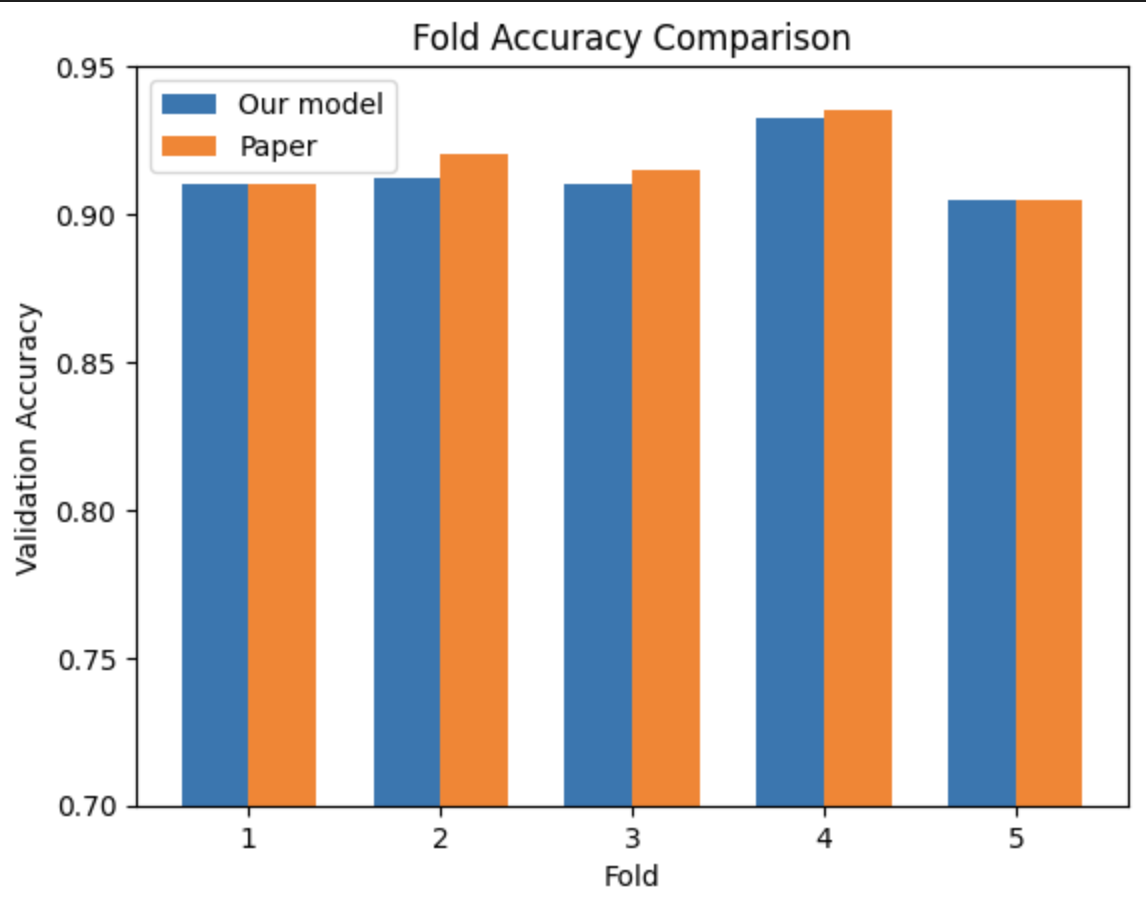
\includegraphics[width=\columnwidth]{image1.png}
\caption{Fold Accuracy Comparison between our model and the original paper. Validation accuracy is compared across five folds.}
\end{figure}

\subsection{Effect of Loss Functions}
While Figure 1 demonstrates the standalone effectiveness of the processing pipeline, we also formally evaluate the isolated contribution of the learning objective. Using exactly the same augmented inputs from the training pipeline, we comprehensively compare identical backbone models optimized dynamically with the three loss strategies: pure cross-entropy loss, supervised contrastive loss, and the joint hybrid loss.

This strict comparison guarantees that all network models universally inherit the benefits of transfer learning and data augmentation. Our key observations confirm that even with a strong training pipeline, the choice of loss function critically impacts performance. While standard cross-entropy successfully focuses on correct classification, it does not explicitly separate classes in the representation space \cite[Sec. II-B]{soundclr}. Conversely, the supervised contrastive loss improves representation quality by actively increasing inter-class separation \cite[Sec. III-C]{soundclr}. 

Ultimately, the joint hybrid objective perfectly merges both advantages \cite[Sec. V]{soundclr}. By optimizing clustering and categorization simultaneously, the hybrid pipeline secures moderately higher categorical accuracy and more consistent results across folds. This effectively demonstrates that the hybrid loss provides a tangible additional improvement on top of the already robust data augmentation pipeline shown in Figure 1.

[to be added figure 2]

\subsection{Implementation Challenges}
Reproducing the paper proved to be more time-consuming than expected. Challenges included setting up the training environment on TAU's Slurm cluster, managing GPU resources, and debugging CUDA compatibility issues. Resource restrictions forced the use of smaller batch sizes than those reported in the paper, affecting training stability and increasing training time. Furthermore, the sheer duration of the training process posed a severe bottleneck: training the unified hybrid or cross-entropy models took approximately one full day per run, while the two-stage supervised contrastive approach (representation learning followed by linear classification) required up to two days. Consequently, any code misconfiguration or systematic error proved exceptionally expensive, often forcing us to restart these prolonged training cycles from scratch.

Additionally, the official repository contained missing dependencies and outdated code that required modification before results could be reproduced reliably. These difficulties highlight the gap between theoretical research and real-world reproducibility.

\section{Results and Discussion}
Our results closely match those reported in the original paper, with differences of approximately $\pm 1\%$ across folds. This slight variance is a strong and expected outcome, well within the margin of acceptable statistical error, naturally arising from non-deterministic GPU operations, data shuffling, and random network initializations. Ultimately, this confirms the correctness of our implementation, the robustness of the method, and the reproducibility of the reported improvements. 

We observe the same key trends outlined by the original authors: the data augmentation and transfer learning pipeline significantly improves baseline performance. Moreover, the hybrid loss provides a tangible additional improvement on top of that pipeline. The combination of supervised contrastive learning and cross-entropy loss acts in a highly complementary manner---where contrastive learning structurally separates class clusters in the embedding space, cross-entropy efficiently refines the decision boundaries---resulting in a reliably positive difference over using either objective alone.

Finally, consistent with the original paper, we observed that the model achieves significantly better accuracy on the ESC datasets (ESC-10 and ESC-50) than it does on the UrbanSound8K (US8K) dataset. While SoundCLR is highly effective on proper ESC benchmarks, this performance disparity across different data distributions raises an important question regarding how the framework can be adapted to achieve stronger generalization across wider, more diverse datasets of unstructured environmental sounds.

\section{Future Work}
A possible improvement is to extend the masking-based augmentation using adaptive masking. Instead of random masking, the model could learn which regions to mask. This could improve robustness and encourage better feature learning, though it would increase complexity and computational cost. Additionally, to improve generalization across diverse datasets like US8K, future work could explore self-supervised contrastive learning on unlabeled audio to train a stronger, dataset-agnostic feature extractor.

\section{Limitations \& Broader Impact}
\textbf{Limitations:} Only part of the original experiments were reproduced due to limited computational resources. Specifically, hardware constraints required using a smaller batch size (64 instead of 128), which slightly limits the negative sample pool for contrastive learning. Furthermore, reproducing the compute-heavy SoundCLR-Ensemble architecture was omitted as it was prohibitively expensive.
\textbf{Broader Impact:} ESC systems are useful in smart environments and assistive technologies. However, they may raise privacy concerns when used in surveillance settings.

\clearpage
\begin{thebibliography}{99}

\bibitem{soundclr}
A. Nasiri and J. Hu, ``SoundCLR: Contrastive Learning of Representations for Improved Environmental Sound Classification,'' \textit{arXiv preprint arXiv:2103.01929}, 2021.

\bibitem{piczak2015esc}
K. J. Piczak, ``ESC: Dataset for Environmental Sound Classification,'' \textit{Proceedings of the 23rd ACM international conference on Multimedia}, 2015.

\bibitem{salamon2017deep}
J. Salamon and J. P. Bello, ``Deep convolutional neural networks and data augmentation for environmental sound classification,'' \textit{IEEE Signal Processing Letters}, vol. 24, no. 3, pp. 279-283, 2017.

\bibitem{salamon2014dataset}
J. Salamon, C. Jacoby, and J. P. Bello, ``A dataset and taxonomy for urban sound research,'' in \textit{Proceedings of the 22nd ACM international conference on Multimedia}, pp. 1041--1044, 2014.

\bibitem{khosla2020supervised}
P. Khosla \textit{et al.}, ``Supervised contrastive learning,'' \textit{Advances in Neural Information Processing Systems}, vol. 33, pp. 18661--18673, 2020.

\bibitem{he2016deep}
K. He, X. Zhang, S. Ren, and J. Sun, ``Deep residual learning for image recognition,'' in \textit{Proceedings of the IEEE conference on computer vision and pattern recognition}, pp. 770--778, 2016.

\bibitem{zhu2018learning}
B. Zhu, C. Wang, F. Liu, J. Lei, Z. Huang, Y. Peng, and F. Li, ``Learning environmental sounds with multi-scale convolutional neural network,'' in \textit{2018 International Joint Conference on Neural Networks (IJCNN)}, pp. 1-8, 2018.

\bibitem{li2007robot}
H. Li, S. Ishikawa, Q. Zhao, M. Ebana, H. Yamamoto, and J. Huang, ``Robot navigation and sound based position identification,'' in \textit{2007 IEEE International Conference on Systems, Man and Cybernetics}, pp. 2394-2399, 2007.

\bibitem{radhakrishnan2005audio}
R. Radhakrishnan, A. Divakaran, and A. Smaragdis, ``Audio analysis for surveillance applications,'' in \textit{IEEE Workshop on Applications of Signal Processing to Audio and Acoustics, 2005.}, pp. 158--161, 2005.

\bibitem{intani2013crime}
P. Intani and T. Orachon, ``Crime warning system using image and sound processing,'' in \textit{2013 13th International Conference on Control, Automation and Systems (ICCAS 2013)}, pp. 1751--1753, 2013.

\bibitem{tokozume2018learning}
Y. Tokozume, Y. Ushiku, and T. Harada, ``Learning from between-class examples for deep sound recognition,'' in \textit{International Conference on Learning Representations}, 2018.

\bibitem{zhang2018deep}
Z. Zhang, S. Xu, S. Cao, and S. Zhang, ``Deep convolutional neural network with mixup for environmental sound classification,'' in \textit{Chinese Conference on Pattern Recognition and Computer Vision (PRCV)}, Springer, pp. 356--367, 2018.

\end{thebibliography}

\end{document}